\subsection{Stochastics}

The lack of a generally valid failure criterion in state-based PD makes an assessment of the initial idea to use a stochastic material distribution for the assessment of failure initiation difficult. However, stochastics may be used to achieve the same entropy in structured discretization as in unstructured base meshes and to individualize failure locations. The comparison of the original hex model with $dx=\SI{0.4}{\milli\meter}$ and horizon $\delta=\SI{1.2}{\milli\meter}$ and three models with stochastic material distribution is shown in \autoref{fig:Results:Hex:Stoch}. Ten different blocks are created with a deviation of the $\SI{2}{\percent}$ of the material bulk and shear modulus.

\pgfplotstableread[col sep=comma]{../../Material/Data/Numerics/Hex_0-4_1-2_Stoch.csv}{\loadedtable}

\begin{figure}[htbp]
  \setlength{\figheight}{7cm}
  \begin{subfigure}{0.55\linewidth}
    \begin{minipage}[b][\figheight]{\linewidth}
    \centering
%     \includegraphics[width=\linewidth,height=\figheight]{example-image-a}
    \tikzexternalenable
    \tikzsetnextfilename{Hex_0-5_0-5625_Stoch}
    \begin{tikzpicture}
      \begin{axis}[
        height=\figheight+\baselineskip,
        width=\linewidth,
        axis lines=middle,
        cycle list name=color list,%linestyles*,
        cycle list shift=1,
        xmin=0,
        ymin=0,
        title=\empty,
        xlabel={Displacement $[\si{\milli\meter}]$},
        ylabel={Force $[\si{\newton}]$},
        x label style={at={(axis description cs:0.5,-0.075)},anchor=north},
        y label style={at={(axis description cs:-0.105,0.5)},rotate=90,anchor=south},
        legend pos=north west,
        legend cell align={left},
        legend style={font=\footnotesize},
      ]%   each nth point={2}
        \addplot+ [thick] table[x=DxNo, y=FxNo] {\loadedtable};
        \addlegendentry{No stochastics}
        \addplot+ [] table[x=DxSto1, y=FxSto1] {\loadedtable};
        \addlegendentry{Stochastic 1}
        \addplot+ [] table[x=DxSto2, y=FxSto2] {\loadedtable};
        \addlegendentry{Stochastic 2}
        \addplot+ [] table[x=DxSto3, y=FxSto3] {\loadedtable};
        \addlegendentry{Stochastic 3}
      \end{axis}
    \end{tikzpicture}
    \tikzexternaldisable
    \end{minipage}
    \caption{Force-displacement plot until failure}
    \label{fig:Results:Tet:Stoch:FD0-5_0-5625}
  \end{subfigure}
  \hfill
  \begin{subfigure}{0.10\linewidth}
    \begin{minipage}[b][\figheight]{\linewidth}
    \centering
      %\includegraphics[angle=90,width=\linewidth,height=\figheight,keepaspectratio]{../../Material/Figures/PD_Hex_Damage_0-4_1-2_3630_-z_ct.png}
      \includegraphics[angle=90,width=\linewidth,height=\figheight,keepaspectratio]{PD_Hex_Damage_0-4_1-2_3630_-z_ct}
    \end{minipage}
    \caption{No}
  \end{subfigure}
  \hfill
  \begin{subfigure}{0.10\linewidth}
    \begin{minipage}[b][\figheight]{\linewidth}
      \centering
      %\includegraphics[angle=90,width=\linewidth,height=\figheight,keepaspectratio]{../../Material/Figures/PD_Hex_Stoch_1_Damage_0-4_1-2_3475_-z_ct.png}
      \includegraphics[angle=90,width=\linewidth,height=\figheight,keepaspectratio]{PD_Hex_Stoch_1_Damage_0-4_1-2_3475_-z_ct}
    \end{minipage}
    \caption{1}
  \end{subfigure}
  \hfill
  \begin{subfigure}{0.10\linewidth}
    \begin{minipage}[b][\figheight]{\linewidth}
      \centering
      %\includegraphics[angle=90,width=\linewidth,height=\figheight,keepaspectratio]{../../Material/Figures/PD_Hex_Stoch_2_Damage_0-4_1-2_3540_-z_ct.png}
      \includegraphics[angle=90,width=\linewidth,height=\figheight,keepaspectratio]{PD_Hex_Stoch_2_Damage_0-4_1-2_3540_-z_ct}
    \end{minipage}
    \caption{2}
  \end{subfigure}
  \begin{subfigure}{0.10\linewidth}
    \begin{minipage}[b][\figheight]{\linewidth}
      \centering
      %\includegraphics[angle=90,width=\linewidth,height=\figheight,keepaspectratio]{../../Material/Figures/PD_Hex_Stoch_3_Damage_0-4_1-2_3292_-z_ct.png}
      \includegraphics[angle=90,width=\linewidth,height=\figheight,keepaspectratio]{PD_Hex_Stoch_3_Damage_0-4_1-2_3292_-z_ct}
    \end{minipage}
    \caption{3}
  \end{subfigure}
  \caption{Failure for hex-mesh with $dx=\SI{0.4}{\milli\meter}$ and stochastics}
  \label{fig:Results:Hex:Stoch}
\end{figure}

It can be seen that the overall stiffness and failure behavior does not change significantly. However, the stochastic material distribution makes it possible to spot several possible individual failure locations. One would expect a less slanted crack propagation. This can be achieved by using a finer discretization. However, a slightly angular failure path can also be observed in tests with a little different specimen geometry of the same material, see \autoref{fig:Results:Exp:AngledCrackPath}. A contact-free displacement measurement using a video extensometer is used to avoid an influence on the crack path.

\begin{figure}
  \centering
  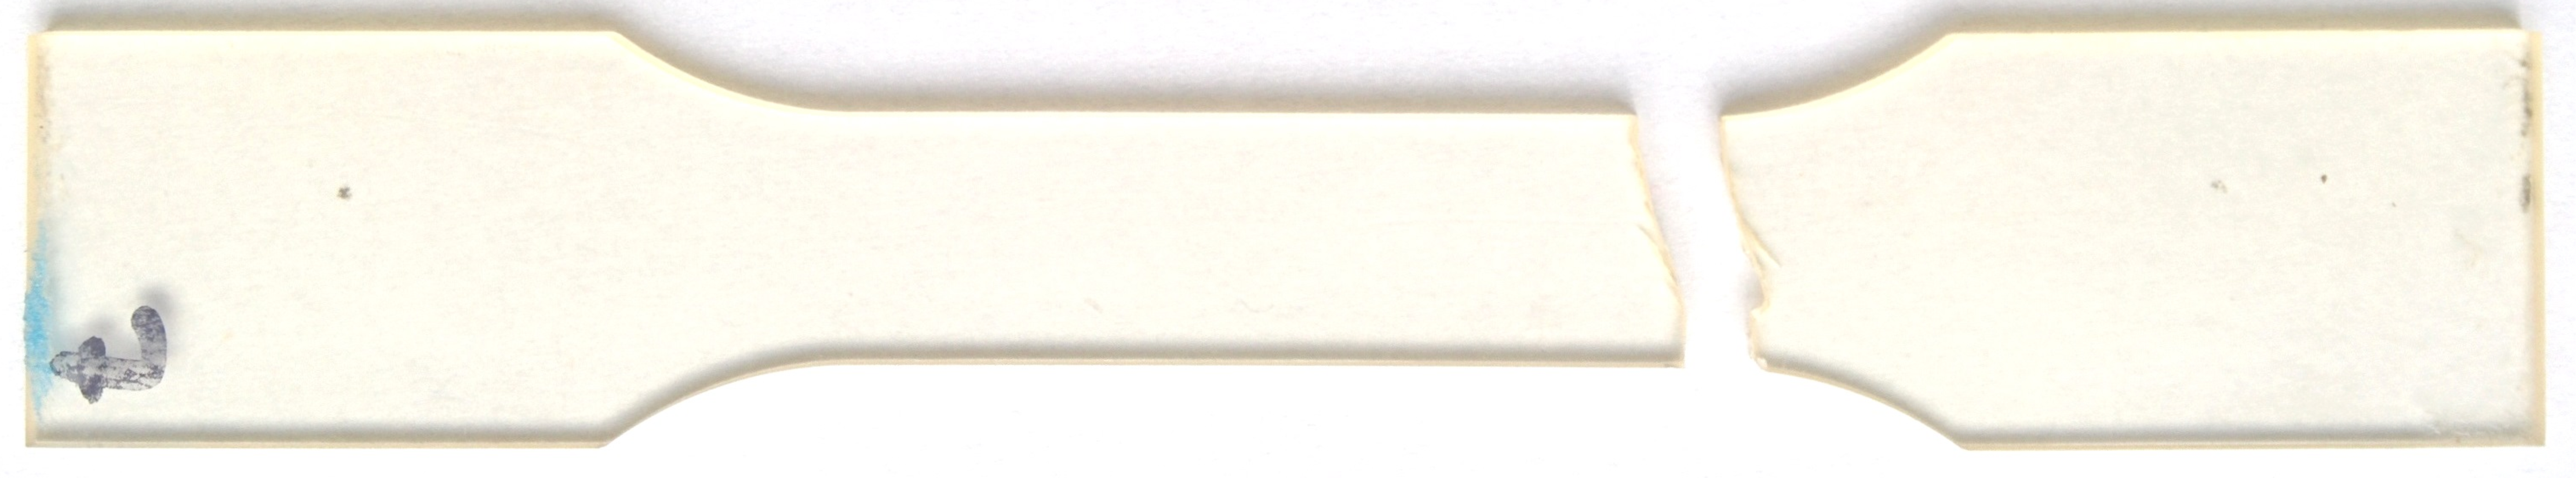
\includegraphics[width=0.5\linewidth,keepaspectratio]{../../Material/Figures/KrauseD_Damage_LY564_statisch}
  \caption{Angled crack path in same material specimen with different geometry \cite{KrauseD2016}}
  \label{fig:Results:Exp:AngledCrackPath}
\end{figure}

The same principal results are valid for tet meshes as shown in \autoref{fig:Results:Tet:Stoch} with a modulus range of $\SI{5}{\percent}$ around the nominal value. It can be noted that the location of failure shifts slightly away from the geometric feature bordering the two separate volumes in this region. In one case failure occurs slightly earlier as a result of the stochastic material distribution. Overall, due to the higher mesh entropy, the effect of stochastic material distribution in tet meshes is smaller than in hex meshes.

\pgfplotstableread[col sep=comma]{../../Material/Data/Numerics/Tet_0-5_0-5625_Stoch.csv}{\loadedtable}

\begin{figure}[htbp]
  \setlength{\figheight}{7cm}
  \begin{subfigure}{0.55\linewidth}
    \begin{minipage}[b][\figheight]{\linewidth}
    \centering
%     \includegraphics[width=\linewidth,height=\figheight]{example-image-a}
    \tikzexternalenable
    \tikzsetnextfilename{Tet_0-4_1-2_Stoch}
    \begin{tikzpicture}
      \begin{axis}[
        height=\figheight+\baselineskip,
        width=\linewidth,
        axis lines=middle,
        cycle list name=color list,%linestyles*,
        cycle list shift=1,
        xmin=0,
        ymin=0,
        title=\empty,
        xlabel={Displacement $[\si{\milli\meter}]$},
        ylabel={Force $[\si{\newton}]$},
        x label style={at={(axis description cs:0.5,-0.075)},anchor=north},
        y label style={at={(axis description cs:-0.105,0.5)},rotate=90,anchor=south},
        legend pos=north west,
        legend cell align={left},
        legend style={font=\footnotesize},
      ]%   each nth point={2}
        \addplot+ [thick] table[x=DxNo, y=FxNo] {\loadedtable};
        \addlegendentry{No stochastics}
        \addplot+ [] table[x=DxSto1, y=FxSto1] {\loadedtable};
        \addlegendentry{Stochastic 1}
        \addplot+ [] table[x=DxSto2, y=FxSto2] {\loadedtable};
        \addlegendentry{Stochastic 2}
        \addplot+ [] table[x=DxSto3, y=FxSto3] {\loadedtable};
        \addlegendentry{Stochastic 3}
      \end{axis}
    \end{tikzpicture}
    \tikzexternaldisable
    \end{minipage}
    \caption{Force-displacement plot until failure}
    \label{fig:Results:Tet:Stoch:FD0-4_1-2}
  \end{subfigure}
  \hfill
  \begin{subfigure}{0.10\linewidth}
    \begin{minipage}[b][\figheight]{\linewidth}
    \centering
      %\includegraphics[angle=90,width=\linewidth,height=\figheight,keepaspectratio]{../../Material/Figures/PD_Tet_Damage_0-5_0-5625_9600_-z_ct.png}
      \includegraphics[angle=90,width=\linewidth,height=\figheight,keepaspectratio]{PD_Tet_Damage_0-5_0-5625_9600_-z_ct}
    \end{minipage}
    \caption{No}
  \end{subfigure}
  \hfill
  \begin{subfigure}{0.10\linewidth}
    \begin{minipage}[b][\figheight]{\linewidth}
      \centering
      %\includegraphics[angle=90,width=\linewidth,height=\figheight,keepaspectratio]{../../Material/Figures/PD_Tet_Stoch_1_Damage_0-5_0-5625_5645_-z_ct.png}
      \includegraphics[angle=90,width=\linewidth,height=\figheight,keepaspectratio]{PD_Tet_Stoch_1_Damage_0-5_0-5625_5645_-z_ct}
    \end{minipage}
    \caption{1}
  \end{subfigure}
  \hfill
  \begin{subfigure}{0.10\linewidth}
    \begin{minipage}[b][\figheight]{\linewidth}
      \centering
      %\includegraphics[angle=90,width=\linewidth,height=\figheight,keepaspectratio]{../../Material/Figures/PD_Tet_Stoch_2_Damage_0-5_0-5625_3950_-z_ct.png}
      \includegraphics[angle=90,width=\linewidth,height=\figheight,keepaspectratio]{PD_Tet_Stoch_2_Damage_0-5_0-5625_3950_-z_ct}
    \end{minipage}
    \caption{2}
  \end{subfigure}
  \begin{subfigure}{0.10\linewidth}
    \begin{minipage}[b][\figheight]{\linewidth}
      \centering
      %\includegraphics[angle=90,width=\linewidth,height=\figheight,keepaspectratio]{../../Material/Figures/PD_Tet_Stoch_3_Damage_0-5_0-5625_3950_-z_ct.png}
      \includegraphics[angle=90,width=\linewidth,height=\figheight,keepaspectratio]{PD_Tet_Stoch_3_Damage_0-5_0-5625_3950_-z_ct}
    \end{minipage}
    \caption{3}
  \end{subfigure}
  \caption{Failure for hex-mesh with $dx=\SI{0.4}{\milli\meter}$ and stochastics}
  \label{fig:Results:Tet:Stoch}
\end{figure}